\section{Main Result: Canonical DR-Plan, Optimality, and Algorithm}
\label{sec:DRP}
% In the problem of the optimal DR-Plan there is generally not a unique plan.
% % Indeed, we will prove a union of $N$ isostatic subgraphs will result in $N$ unique plans, but that at the $N^{\text{th}}$ level of the tree it will always be the same. Therefore, all choices of decomposition are in some sense equivalent. The theorem we seek to prove is thus:
% However, we will show that regardless of which children are chosen for the plan, so long as they satisfy the definition of an optimal DR-plan, the recombination will require solving of the same systems. Being the smallest such structure that offers this, the definition of an optimal DR-plan could be considered the canonical DR-plan.
% % To assist in showing this, we prove this core theorem throughout this section:

% In this section, we discuss 2D bar-joint graphs. All vertex weights are $2$, all edge weights are $1$, and constant $k= -{{3}\choose{2}}=-3$. Trivial graphs are a single vertex and empty set. Furthermore, 2D isostatic graphs must be connected.
% % The greatest density of a 2D isostatic graph is $-2$ (the vertex). The other disconnected part of the graph would need to have a density of $-1$, which is overconstrained and not possible in a isostatic graph (because there is no trivial graph with that density).


\subsection{Canonical DR-Plan}
In this section, we define a \dfn{canonical} plan to capture those aspects of an optimal DR-plan that mimic the  uniqueness of a complete DR-plan, and we show that the nonunique aspects do not affect optimality for independent (underconstrained or isostatic) graphs. Furthermore, we give an efficient \ComplexityCanDRP\ algorithm to find the canonical DR-plan of any independent graph. The definition is as follows:


% \begin{definition}\label{def:canonical_drplan}
%     The \dfn{canonical DR-plan} of a graph $G$ satisfies the following three properties:
%     (1) it is a DR-plan of $G$;
%     (2) children are rigid vertex-maximal proper subgraphs of the parent; and
%     (3) if all pairs of rigid vertex-maximal proper subgraphs intersect trivially then all of them are children, otherwise exactly two that intersect non-trivially are children.
% \end{definition}

\begin{definition}\label{def:canonical_drplan}
    A \dfn{canonical DR-plan} is a DR-plan that satisfies the additional two properties:
    \begin{enumerate}
        \item Children are rigid vertex-maximal proper subgraphs of the parent.
        \item If all pairs of rigid vertex-maximal proper subgraphs intersect trivially then all of them are children, otherwise exactly two that intersect non-trivially are children.
    \end{enumerate}
\end{definition}


In this section and in section~\ref{sec:recomb}, any reference to a graph $G$ is assumed to be isostatic (i.e.\ well-constrained or $(k,l)$-tight).
% \sidenote{In this section, $G$ is always assumed to be isostatic.}



% This definition gives the canonical DR-plan a surprisingly strong Church-Rosser property.

Definition~\ref{def:canonical_drplan} gives the canonical DR-plan a surprisingly strong Church-Rosser property, which is made explicit in Theorem~\ref{theorem:main}, the main result of this section.

\begin{theorem}
\label{theorem:canonical_exists_and_is_optimal}
\label{theorem:canonical_is_optimal}
\label{theorem:main}
    A canonical DR-plan exists for a graph $G$ and any canonical DR-plan is optimal if $G$ is independent.
\end{theorem}


% \begin{theorem} \label{theorem:canonical_is_optimal}
%     \label{theorem:main}
%     Any canonical DR-plan is an optimal DR-plan.
% \end{theorem}

%The proof of this theorem is a direct consequence of the following  more general theorem.

%\begin{theorem}\label{theorem:main}
%Given an isostatic 2D bar-joint graph $G$ and ComDRP$(G)$, for all nodes $C$
%with children $C_1,\ldots,C_N$ preserve children according to the following rules.
%\begin{enumerate}
%    \item If $C_i \cap C_j$ is trivial then keep all $C_1,\ldots,C_N$ as children.
%    \item If $C_i \cap C_j$ is isostatic then select any two out of $C_1,\ldots,C_N$ as children.
%\end{enumerate}
%This is a canonical DR-plan.
%\end{theorem}


\begin{proof}
We show the existence of a canonical DR-plan by constructing it as follows:

Begin with $\comdrp{G}$ of a rigid 2D bar-joint graph $G$, for all nodes $C$ with children $C_1,\ldots,C_N$  retain children nodes according to the following rules:
\begin{enumerate}
   \item If $C_i \cap C_j$ is trivial then retain all $C_1,\ldots,C_N$ as children.
   \item If $C_i \cap C_j$ is rigid then select any two out of $C_1,\ldots,C_N$ as children.
\end{enumerate}

This directly satisfies Properties (2) and (3) of a canonical DR-plan (see Definition~\ref{def:canonical_drplan}), because all the nodes in $\comdrp{G}$ are rigid vertex-maximal proper subgraphs,  which we shorten to {\em clusters}.  To show Property (1) holds (that this constitutes a DR-plan):
for Case 1 above,  since we start with a complete DR-plan, if we preserve all the children it is still a DR-plan; for Case 2 above, we know that the union must be rigid as well and it cannot be anything other than $C$, otherwise we would have found a larger rigid proper subgraph of $C$, contradicting vertex-maximality.

Note that if we begin with an isostatic graph, ``rigid'' can be replaced with ``isostatic'' throughout the construction and preserve the above properties. The rigid proper subgraphs of an isostatic graph must be isostatic themselves.

Next we show that a canonical DR-plan is optimal.

First, note  that any  DR-plan $R$ without the Property (2) of a canonical DR-plan can always be modified (by introducing intermediate nodes) to satisfy Property (2) without  increasing the max fan-in, since any rigid proper subgraph of a graph $C$ (a child of node $C$ of the DR-plan $R$)
is the subgraph of some cluster of $C$.
Thus without loss of generality, we can assume that an optimal DR-plan satisfies Property (2) of a canonical DR-plan.

The proof of optimality of a canonical DR-plan is by induction on its height.  The base case trivially holds for canonical DR-plans of height 0, i.e.\ for single edges. The induction hypothesis is that canonical DR-plans of height $t$ are optimal for the root node.
For the induction step consider a canonical DR-plan $R$ of  height $t+1$ rooted at a node $C$.
Notice that $R$ represents a canonical DR-plan $R(C)$ for the graphs $C$ corresponding to each of its  descendant nodes.
Thus, from the induction hypothesis, we know that the $R(C_i)$ is optimal for $C_i$.

Thus it is sufficient to demonstrate a set of nodes $S$  that must be present in any  DR-plan $R$ for $C$ that satisfies Property (2), including a known optimal one; and furthermore, for any such DR-plan $R$,  either (Claim 1) $S$ must be the set of children of $C$; or (Claim 2) for all the ancestors $A$ of $S$, $R$ has the minimum possible fan-in of 2.

We show the two claims below.
The first claim is that for a node $C$ whose clusters have trivial pairwise intersections, any DR-plan of $C$ that satisfies Property (2) must also satisfy Property (3) at $C$, i.e.\ the set of children $S$ of $C$ consists of all clusters of $C$.
Because this is the only choice, it is the minimum fan-in at $C$ for any DR-plan for $C$ with Property (2), including a known optimal one.
The second claim shows that in the case of nodes $C$ whose rigid, vertex-maximal proper subgraphs have  non-trivial pairwise intersections, every canonical DR-plan of $C$ that uses any possible choice of two such subgraphs of $C$ as children results in a minimum possible fan-in of 2 in the ancestor nodes $A$ leading to the {\em same maximal antichain $S$ of descendants $D$ of $C$}. The antichain is maximal in the partial order of rigid subgraphs of $C$ under containment. I.e.\ $S$ satisfies the property that every proper vertex-maximal rigid subgraph of $C$ is a superset of some $D$ in $S$; this follows from properties of maximal antichains that no element of $S$ is contained in the union of other elements of $S$; and the union of elements of $S$ is $C$. Thus any  DR-plan that satisfies Property (2) and hence contains two or more of the rigid vertex-maximal proper subgraphs of $C$ as children must also contain every element of $S$. The two claims complete the proof that every canonical DR-plan is optimal.



 % We do this inductively on the l, beginning with the root node, showing that the rules are always the optimal choice.
% by discussing each rule and proving inductively that this is the optimal choice at each level of the DR-plan tree, starting with the root node.


% Now we show that this plan is optimal by considering the two cases. Observation \ref{lemma:union_intersection} shows that we do not have to consider anything other than the two cases stated in the construction.
 % the intersection of any two isostatic subgraphs can only result in trivial or isostatic subgraphs. Therefore, given $C$ and its isostatic vertex-maximal subgraphs $C_1,\ldots,C_N$, the are only two possibilities to consider. Either (1) subgraphs $C_i$ and $C_j$ have a trivial intersection, or (2) they have an isostatic intersection.





\medskip\noindent
\vemph{Claim 1:}
% If some pair is intersecting trivially, then in fact all pairs intersect trivially, thus all must be children by defn of canonical drplan
%
A set of clusters $C_1,\ldots,C_N$ whose pairwise intersection is trivial, must be children of $C$ in an optimal DR-plan.

We prove this claim  by showing that the union of no subset of the children can be $C$, thereby requiring all of them to be included as children.


% must be optimal for this node.

We prove by contradiction.
Assume to the contrary that the strict subset $S\subsetneq \{1,\ldots,N\}$ such that $U=\bigcup_{i\in S}{C_i}$ is isostatic. If $U\neq C$, then we found a larger proper subgraph contradicting vertex-maximality of the $C_i$. So, it must be that $U=C$.
\usestwod
However, since $C_i \cap C_j$ is trivial then for $k\notin S$ we know, by Lemma \ref{lemma:combined_lemma}, Item \ref{lemma:uc_intersection_makes_all_uc}, $U\cap C_k$ must be one or more trivial, i.e.\ disconnected vertices. By definition of a DR-plan, $C_k=C\cap C_k$ and we know that $U=C$ so $C_k=U\cap C_k$. Thus, $C_k$ is (i) a collection of disconnected vertices, and (ii) an isostatic subgraph of $C$, which is impossible. As $C$ is isostatic, this means the union of no proper subset of $C_1,\ldots,C_N$ is isostatic, nor is it equal to $C$, proving Claim 1.

Furthermore, since a canonical DR-plan has nodes with proper rigid \vemph{vertex-maximal} subgraphs as children, if, as in this case, their pairwise intersection is trivial, it follows that any node has at most as many children as a DR-plan without this restriction, because the union of the children must contain all edges of the parent. Therefore, the canonical DR-plan is the optimal choice in this case of trivial intersections.

\medskip\noindent
\vemph{Claim 2:}
If some pair in the set of child clusters $C_1,\ldots,C_N$ of $C$ has an isostatic (nontrivial) intersection, then choosing any two as children (minimum possible fan-in) will result in the same maximal antichain of descendants of $C$.

To prove Claim 2, notice that if  $C_i \cap C_j$ is isostatic, then, by Observation \ref{lemma:union_intersection}, $C_i \cup C_j$ is also isostatic. This means that, by Lemma \ref{lemma:combined_lemma}, Point \ref{lemma:wc_intersection_makes_all_wc}, the union of any two children of $C$ is $C$ itself. Thus, any two children can be chosen to make a canonical DR-plan and that is the minimum fan-in possible for a node of the DR-plan.
% are potential choices for the optimal DR-plan as they all create equal fan-in (exactly two) at this level.

\newcommand{\induceonc}[1]{Idc\left(C,#1\right)}
\renewcommand{\induceonc}[1]{#1}
\newcommand{\iunion}[1]{\induceonc{I\cup\bigcup_{k\in [N]\setminus\{#1\}}{R_k}}}

However, to guarantee that any two are the \vemph{optimal} choice, it must ensure minimum fan-in over all descendants leading up to a common maximal antichain $S$ of subgraphs.

To prove this holds, take the set $[N]=\{1,\dots,N\}$, and denote $I=\bigcap_{k\in [N]}{C_k}$ and $R_k=C\setminus C_k$. Suppose  $C_i$ and $C_j$, where $i\neq j$,  are  the children. For convenience, we will assume all subgraphs are induced subgraphs of $C$. We know that $C=\induceonc{I\cup\bigcup_{k\in [N]}{R_k}}$ and $C_i=\iunion{i}$. The isostatic vertex-maximal subgraphs of $C_i$ are $(\iunion{i,1}),\ldots,(\iunion{i,i-1}),(\iunion{i,i+1}),\ldots,(\iunion{i,N})$ all of whose pairwise intersections are isostatic subgraphs. So any two of these are viable children for $C_i$.
% Since
% \[C_i=Idc\left(C,I\cup\bigcup_{k\in S_N\setminus\{i\}}{R_k}\right)\]
% the children of $C_i$ will be
% \[Idc\left(C,I\cup\bigcup_{k\in S_N\setminus\{i,m\}}{R_k}\right)\]
% and
% \[Idc\left(C,I\cup\bigcup_{k\in S_N\setminus\{i,n\}}{R_k}\right)\]
% % $C_i=Idc\left(C,I\cup\bigcup_{k\in S_N\setminus\{i\}}{R_k}\right)$
% % the children of this node will be
% % $Idc\left(C,I\cup\bigcup_{k\in S_N\setminus\{i,m\}}{R_k}\right)$
% % and
% % $Idc\left(C,I\cup\bigcup_{k\in S_N\setminus\{i,n\}}{R_k}\right)$
% for arbitrary $m$ and $n$, where $i,j,m,n$ do not equal each other. \todo{Prove these are valid children? Or is this obvious?}
This continues for $N-1$ levels, always with fan-in of two (the minimum possible), at which point every descendant of $C$ is some $\induceonc{I\cup R_k}$ for $k\in [N]$, with every $k$ appearing at least once. At the last level, there are exactly two rigid proper vertex-maximal subgraphs, and hence a unique choice of pair of children. Thus, regardless of the sequence of choices of $C_i$ and $C_j$, and of their descendants at each level, the DR-plan has the optimal fan-in of two for every node for  $N$ levels,  and the collection of last level nodes contain the same maximal antichain of subgraphs (for all choices).
%
% \medskip\noindent
% This proof then applies to itself recursively to show that the fan-in of the children will also be minimum.
%
% -- say this at top `proof is by induction on the level of the dr=plan'
\end{proof}

This proof of this theorem relies on the following crucial observation and lemma. These will be used again in the application sections (\ref{sec:bodypin} and \ref{sec:pinnedline}) of the paper, with modifications to work for other types of qusecs.

\begin{observation*}\label{lemma:union_intersection}
If $F_i$ and $F_j$ are non-empty isostatic graphs then the following hold: \\
(1) $F_i\cup F_j$ is not trivial;
(2) $F_i\cup F_j$ is underconstrained if and only if $F_i\cap F_j$ is trivial;
(3) $F_i\cup F_j$ is isostatic if and only if $F_i\cap F_j$ is isostatic; and
(4) $F_i\cap F_j$ is not underconstrained.
\end{observation*}

The following key properties hold at the nodes of a canonical DR-plan.

\begin{lemma*}\label{lemma:combined_lemma}
Let $C$ be an isostatic node of a canonical DR-plan, with distinct children $C_1,C_2,\ldots, C_m$. Assume $i\ne j$.
Then
\begin{enumerate}
    \item\label{lemma:wc_intersection_is_C}
    $C_i\cup C_j$ is isostatic if and only if $C_i\cup C_j = C$.

    \item\label{lemma:wc_intersection_makes_all_wc}
    If $C_i\cup C_j$ is isostatic, then $\forall k: C_i\cup C_k$ is isostatic. Alternatively, if $C_i\cup C_j=C$, then $\forall k: C_i\cup C_k=C$.

    \item\label{lemma:uc_intersection_makes_all_uc}
    If $C_i\cap C_j$ is trivial, then $\forall k: C_i\cap C_k$ is trivial.
\end{enumerate}
\end{lemma*}

\begin{remark}
The first item in the above lemma generalizes to the union of any number of children, $C_1,\ldots,C_k$, resulting in the desirable property of \dfn{cluster minimality} (defined in \cite{hoffman2001decompositionI} and in Section \ref{sec:prev}) holding for canonical-optimal DR-plans.
\end{remark}





% \begin{figure*}\centering
% \begin{subfigure}{.3\linewidth}\centering
%     % \newcommand{\tedge}[5]{\draw[#3] (#1)-- node[e, #5] (e#4) {#4} (#2)}

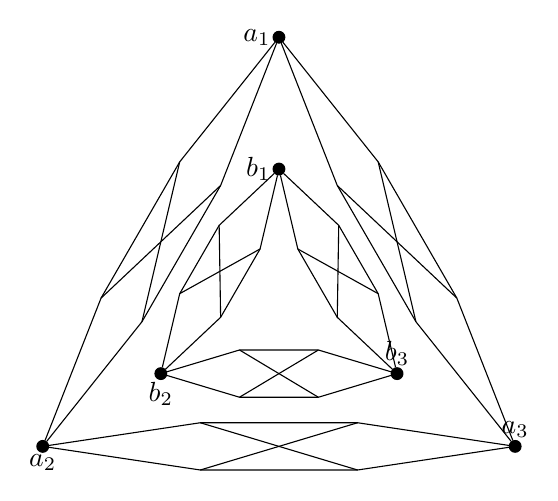
\begin{tikzpicture}[scale=3]
    \tikzstyle{v}=[draw, circle, minimum size=0.75cm]
    \tikzstyle{c}=[draw, circle, inner sep=1.5, fill=black]
    \tikzstyle{e}=[]

    \node[circle,fill=white,inner sep=7] (center) at (0,0-.125-.1) {};

    \node[c] (v1) at (0,0.866) [label={left,inner sep=.555}:$a_1$]{};
    \node[c] (v2) at (-1,-0.866) [label={below,inner sep=.555}:$a_2$]{};
    \node[c] (v3) at (1,-0.866) [label={above,inner sep=.555}:$a_3$]{};

    \node[c] (v4) at (0,0.433-.125) [label={left,inner sep=.555}:$b_1$]{};
    \node[c] (v5) at (-0.5,-0.433-.125) [label={below,inner sep=.555}:$b_2$]{};
    \node[c] (v6) at (0.5,-0.433-.125) [label={above,inner sep=.555}:$b_3$]{};

    \tedge{v1}{v2}{solid}{}{};
    \tedge{v1}{v3}{solid}{}{};
    \tedge{v2}{v3}{solid}{}{};

    \tedge{v4}{v5}{solid}{}{};
    \tedge{v4}{v6}{solid}{}{};
    \tedge{v5}{v6}{solid}{}{};


    \tedge{v1}{v4}{solid}{}{};
    \tedge{v2}{v5}{solid}{}{};
    \tedge{v3}{v6}{solid}{}{};


    \tedge{v4}{center}{dashed}{}{};
    \tedge{v5}{center}{dashed}{}{};
    \tedge{v6}{center}{dashed}{}{};


    % sin(30deg) = 0.5
    % cos(30deg) = 0.866

    % o/i -> outside/inside triangle
    % b/l/r -> bottom/left/right edge of triangle

    \coordinate (ob0) at (-0.333,-0.866-0.1);
    \coordinate (ob1) at (0.333,-0.866-0.1);
    \coordinate (ob2) at (-0.333,-0.866+0.1);
    \coordinate (ob3) at (0.333,-0.866+0.1);
    \draw (v2) -- (ob0) -- (ob1) -- (v3);
    \draw (v2) -- (ob2) -- (ob3) -- (v3);
    \draw (ob0) -- (ob3);
    \draw (ob2) -- (ob1);

    \draw[rotate around={60:(-1,-0.866)}] (v2) -- (-0.333,-0.766) -- (0.333,-0.766) -- (v1);
    \draw[rotate around={60:(-1,-0.866)}]  (v2) -- (-0.333,-0.966) -- (0.333,-0.966) -- (v1);
    \draw[rotate around={60:(-1,-0.866)}]  (-0.333,-0.766) -- (0.333,-0.966);
    \draw[rotate around={60:(-1,-0.866)}]  (-0.333,-0.966) -- (0.333,-0.766);

    \draw[rotate around={-60:(1,-0.866)}] (v3) -- (0.333,-0.766) -- (-0.333,-0.766) -- (v1);
    \draw[rotate around={-60:(1,-0.866)}]  (v3) -- (0.333,-0.966) -- (-0.333,-0.966) -- (v1);
    \draw[rotate around={-60:(1,-0.866)}]  (-0.333,-0.766) -- (0.333,-0.966);
    \draw[rotate around={-60:(1,-0.866)}]  (-0.333,-0.966) -- (0.333,-0.766);




    \coordinate (ib0) at (-0.167,-0.433-.125-0.1); %(-.167,-.658)
    \coordinate (ib1) at (0.167,-0.433-.125-0.1); %(.167,-.658)
    \coordinate (ib2) at (-0.167,-0.433-.125+0.1);%(-.167,-.458)
    \coordinate (ib3) at (0.167,-0.433-.125+0.1);%(.167,-.458)
    \draw (v5) -- (ib0) -- (ib1) -- (v6);
    \draw (v5) -- (ib2) -- (ib3) -- (v6);
    \draw (ib0) -- (ib3);
    \draw (ib2) -- (ib1);

    \draw[rotate around={60:(-0.5,-0.558)}] (v5) -- (-.167,-.658) -- (.167,-.658) -- (v4);
    \draw[rotate around={60:(-0.5,-0.558)}]  (v5) -- (-.167,-.458) -- (.167,-.458) -- (v4);
    \draw[rotate around={60:(-0.5,-0.558)}]  (-.167,-.658) -- (.167,-.458);
    \draw[rotate around={60:(-0.5,-0.558)}]  (-.167,-.458) -- (.167,-.658);

    \draw[rotate around={-60:(0.5,-0.558)}] (v6) -- (.167,-.658) -- (-.167,-.658) -- (v4);
    \draw[rotate around={-60:(0.5,-0.558)}]  (v6) -- (.167,-.458) -- (-.167,-.458) -- (v4);
    \draw[rotate around={-60:(0.5,-0.558)}]  (-.167,-.658) -- (.167,-.458);
    \draw[rotate around={-60:(0.5,-0.558)}]  (-.167,-.458) -- (.167,-.658);
% \newcommand{\tedge}[5]{\draw[#3] (#1)-- node[e, #5] (e#4) {#4} (#2)}

    % \draw (-1,-0.866) -- (-0.333,-0.966);

\end{tikzpicture}

%     \caption{}\label{fig:c2c3ofk33s:a}
% \end{subfigure}%
% \begin{subfigure}{.7\linewidth}\centering
%     % \newcommand{\tedge}[5]{\draw[#3] (#1)-- node[e, #5] (e#4) {#4} (#2)}

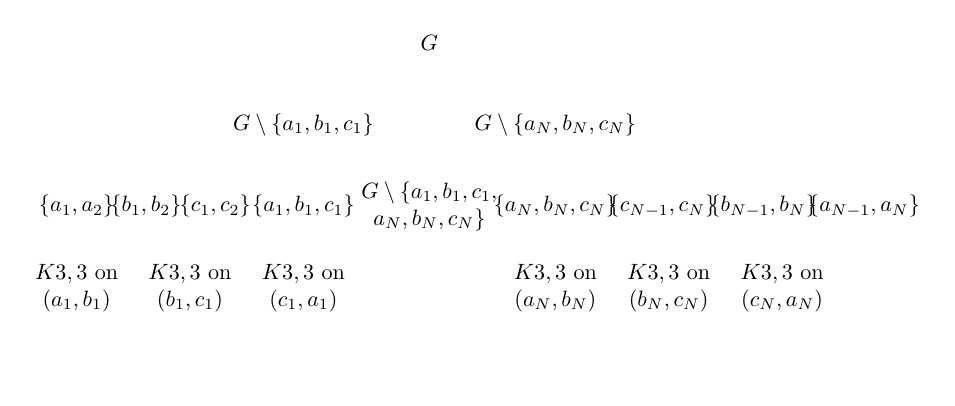
\begin{tikzpicture}[scale=.8, transform shape]
    \tikzstyle{v}=[draw, circle, minimum size=0.75cm, font=\footnotesize]
    % \tikzstyle{b}=[draw, font=\footnotesize]
    \tikzstyle{b}=[align=center]
    \tikzstyle{e}=[]

    \node[b] (c0) at (0,0*1.3) {$G$};
    \node[b] (c1a) at (-2,-1*1.3) {$G\setminus\{a_1,b_1,c_1\}$};
    \node[b] (c1b) at (2,-1*1.3) {$G\setminus\{a_N,b_N,c_N\}$};
    \node[b] (c2b) at (0,-2*1.3) {$G\setminus\{a_1,b_1,c_1,$ \\ $a_N,b_N,c_N\}$};
    \node[b] (c2a) at (-2,-2*1.3) {$\{a_1,b_1,c_1\}$};
    \node[b] (c2c) at (2,-2*1.3) {$\{a_N,b_N,c_N\}$};
    \node[b] (c2ab1) at (-5.6,-2*1.3) {$\{a_1,a_2\}$};
    \node[b] (c2ab2) at (-4.5,-2*1.3) {$\{b_1,b_2\}$};
    \node[b] (c2ab3) at (-3.4,-2*1.3) {$\{c_1,c_2\}$};
    \node[b] (c2bc1) at (6.9,-2*1.3) {$\{a_{N-1},a_N\}$};
    \node[b] (c2bc2) at (5.3,-2*1.3) {$\{b_{N-1},b_N\}$};
    \node[b] (c2bc3) at (3.7,-2*1.3) {$\{c_{N-1},c_N\}$};

    \node[b] (ab1k33) at (-5.6,-3*1.3) {$K3,3$ on \\ $(a_1,b_1)$};
    \node[b] (bc1k33) at (-7.6/2,-3*1.3) {$K3,3$ on \\ $(b_1,c_1)$};
    \node[b] (ca1k33) at (-2,-3*1.3) {$K3,3$ on \\ $(c_1,a_1)$};

    \node[b] (abNk33) at (2,-3*1.3) {$K3,3$ on \\ $(a_N,b_N)$};
    \node[b] (bcNk33) at (7.6/2,-3*1.3) {$K3,3$ on \\ $(b_N,c_N)$};
    \node[b] (caNk33) at (5.6,-3*1.3) {$K3,3$ on \\ $(c_N,a_N)$};


    \node[b] (c3a) at (-2,-4*1.3) {};
    \node[b] (c3b) at (2,-4*1.3) {};


    \tedge{c0}{c1a}{solid}{}{};
    \tedge{c0}{c1b}{solid}{}{};

    \tedge{c1a}{c2ab1}{solid}{}{};
    \tedge{c1a}{c2ab2}{solid}{}{};
    \tedge{c1a}{c2ab3}{solid}{}{};
    \tedge{c1a}{c2a}{solid}{}{};
    \tedge{c1a}{c2b}{solid}{}{};

    \tedge{c1b}{c2bc1}{solid}{}{};
    \tedge{c1b}{c2bc2}{solid}{}{};
    \tedge{c1b}{c2bc3}{solid}{}{};
    \tedge{c1b}{c2b}{solid}{}{};
    \tedge{c1b}{c2c}{solid}{}{};

    \tedge{c2a}{ab1k33}{solid}{}{};
    \tedge{c2a}{bc1k33}{solid}{}{};
    \tedge{c2a}{ca1k33}{solid}{}{};
    \tedge{c2c}{abNk33}{solid}{}{};
    \tedge{c2c}{bcNk33}{solid}{}{};
    \tedge{c2c}{caNk33}{solid}{}{};

    \tedge{c2b}{c3a}{dashed}{}{};
    \tedge{c2b}{c3b}{dashed}{}{};
\end{tikzpicture}

%     \caption{}\label{fig:c2c3ofk33s:b}
% \end{subfigure}

% \caption{(\ref{fig:c2c3ofk33s:a}) A doublet ($C_2 \times C_3$) with each edge of the triangles replaced by a $K_{3,3}$. This pattern continues inwards for a total of $N$ triangles, indicated by the dashed lines. (\ref{fig:c2c3ofk33s:b}) Most of the DR-plan of this graph, omitting further decomposition of $K_{3,3}$ subgraphs into the separate 9 edges and of edges into the component nodes. $G\setminus\{a_i,b_i,c_i\}$ is shorthand for $G$ difference those nodes and all of the nodes in the corresponding $K_{3,3}$ subgraphs. The dashed lines indicated that this exact structure is repeated.}
% \label{fig:c2c3ofk33s}
% \end{figure*}


% \FigInit
%     {(\ref{fig:c2c3ofk33s:a}) A doublet ($C_2 \times C_3$) with each edge of the triangles replaced by a $K_{3,3}$. This pattern continues inwards for a total of $N$ triangles, indicated by the dashed lines. (\ref{fig:c2c3ofk33s:b}) Most of the DR-plan of this graph, omitting further decomposition of $K_{3,3}$ subgraphs into the separate 9 edges and of edges into the component nodes. $G\setminus\{a_i,b_i,c_i\}$ is shorthand for $G$ difference those nodes and all of the nodes in the corresponding $K_{3,3}$ subgraphs. The dashed lines indicated that this exact structure is repeated.}
%     {fig:c2c3ofk33s}
% \FigTwoSubfigWithWidth
%     {.3}
%     {../../img/epsfromtikz/c2c3_of_k33s-0}
%     {}
%     {fig:c2c3ofk33s:a}
%     %
%     {.7}
%     {../../img/epsfromtikz/c2c3_of_k33s-1}
%     {}
%     {fig:c2c3ofk33s:b}


% \ClearMyMinHeight
% \SetMyMinHeight{.3}{../../img/epsfromtikz/c2c3_of_k33s-0}
% \SetMyMinHeight{.7}{../../img/epsfromtikz/c2c3_of_k33s-1}

% \begin{figure*}\centering%
%     %
%     \begin{subfigure}{0.3\linewidth}\centering
%         \includegraphics[height=\myMinHeight]{../../img/epsfromtikz/c2c3_of_k33s-0}
%         \caption{}\label{fig:c2c3ofk33s:a}
%     \end{subfigure}%
%     %
%     \hfill
%     \begin{subfigure}{0.7\linewidth}\centering
%         \includegraphics[height=\myMinHeight]{../../img/epsfromtikz/c2c3_of_k33s-1}
%         \caption{}\label{fig:c2c3ofk33s:b}
%     \end{subfigure}%
%     %
%     \caption{(\ref{fig:c2c3ofk33s:a}) A doublet ($C_2 \times C_3$) with each edge of the triangles replaced by a $K_{3,3}$. This pattern continues inwards for a total of $N$ triangles, indicated by the dashed lines. (\ref{fig:c2c3ofk33s:b}) Most of the DR-plan of this graph, omitting further decomposition of $K_{3,3}$ subgraphs into the separate 9 edges and of edges into the component nodes. $G\setminus\{a_i,b_i,c_i\}$ is shorthand for $G$ difference those nodes and all of the nodes in the corresponding $K_{3,3}$ subgraphs. The dashed lines indicated that this exact structure is repeated.}
%     \label{fig:c2c3ofk33s}
% \end{figure*}%

\ClearMyMinHeight
\SetMyMinHeight{.3}{../../img/svg/revised_c2c3_of_k33s}
\SetMyMinHeight{.7}{../../img/svg/revised_c2c3_of_k33s_candrp}

\begin{figure*}\centering%
    %
    \begin{subfigure}{0.3\linewidth}\centering
        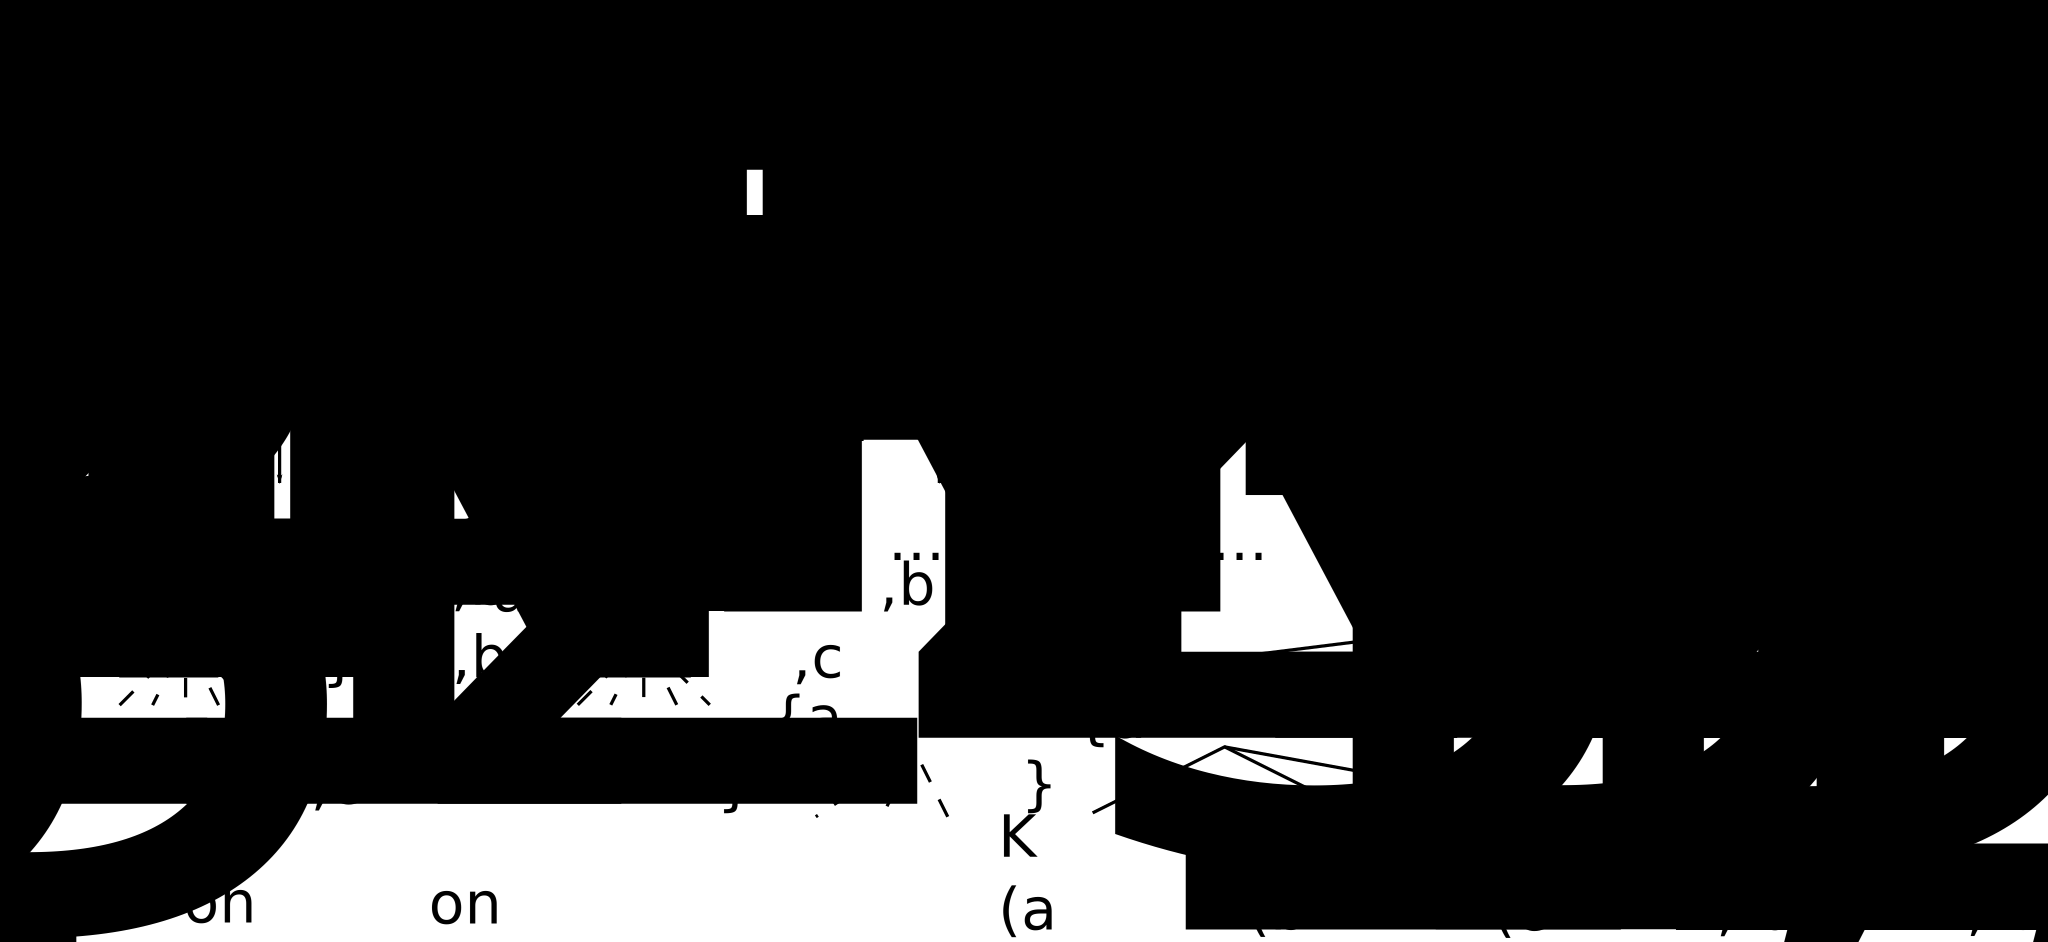
\includegraphics[height=\myMinHeight]{../../img/svg/revised_c2c3_of_k33s}
        \caption{}\label{fig:c2c3ofk33s:a}
    \end{subfigure}%
    %
    \hfill
    \begin{subfigure}{0.7\linewidth}\centering
        \includegraphics[height=\myMinHeight]{../../img/svg/revised_c2c3_of_k33s_candrp}
        \caption{}\label{fig:c2c3ofk33s:b}
    \end{subfigure}%
    %
    \caption{
    (\ref{fig:c2c3ofk33s:a}) A sequence of doublets ($C_2 \times C_3$) intersecting on triangles, where the edges of the triangles are replaced by $K_{3,3}$'s. This pattern continues inwards for a total of $N$ triangles, indicated by the dashed arrows. (\ref{fig:c2c3ofk33s:b}) The canonical DR-plan of $G$, drawn as a DAG. $G\setminus\{a_i,b_i,c_i\}$ is shorthand for $G$ difference those nodes and all of the nodes in the corresponding $K_{3,3}$ subgraphs. Below the third level, the obvious pattern continues until only the individual doublets are present (fourth level) with the ellipses indicating the remaining doublets between those shown. Decomposition of one of these doublets is shown. The dashed lines indicated that this exact decomposition (of the similar nodes on the level) is repeated. Further decomposition of $K_{3,3}$ subgraphs into the separate 9 edges is omitted from the figure.
    }
    \label{fig:c2c3ofk33s}
\end{figure*}%




\begin{example}[DR-plan for self-similar structure]
% \myexample
% \textsl{[DR-plan for self-similar structure]}
This example details the decomposition of the graph in Figure \ref{fig:c2c3ofk33s}, the canonical DR-plan of $G$. It begins with the whole (isostatic) graph as the root. The graph $G$ has only two isostatic vertex-maximal subgraphs: $G$ without the outermost triangle composed of $K_{3,3}$ graphs (triangle $1$) and $G$ without the inner triangle (triangle $N$). These intersect on $G$ without triangle $1$ and $N$ which is clearly isostatic. As explained in the proof of Theorem \ref{theorem:main}, since there are only 2 possible children, their intersection must be a node 2 levels below the parent. As expected, it is on the third level, as a child of both of $G$'s children.

Both of $G$'s children are similar to $G$, but containing only $N-1$ triangles. Therefore, the canonical DR-plans of these children follow the same pattern. This continues downward until the individual doublets are reached (there will be multiple occurrences of the same doublets at this level, but they can be represented as the same node in a DAG).

Further decomposition of one of these doublets is shown. The three edges between the triangles and the triangles themselves all intersect trivially pairwise. By Theorem \ref{theorem:main}, part 1, they must all be children in the DR-plan. Similarly, the triangles decompose into their three trivially intersecting $K_{3,3}$'s. Then the $K_{3,3}$ subgraphs decompose into their separate 9 edges.

The self-similar nature of this graph is evident in the canonical DR-plan. Many structures are repeated throughout the DR-plan, allowing for shared computation in both decomposition and recombination.
\end{example}




% \subsection{Extensions}
% This framework immediately pushes through for body-pin systems via a simple reduction. If there are $N$ pins on a body, it can be represented as a 2-tree with $N$ vertices, each corresponding to a pin, making sure to select edge distances such that the distance between pins is preserved. E.g.\ a body with two pins is an edge, three pins is a triangle, etc. Any bodies that share a pin now intersect on their vertex that corresponds to that pin. Now we have a bar-joint representation of the body-pin system in 2D and all proofs follow.

% With more effort, it can be shown that pinned line-incidence systems can also use this framework. This is done in section \ref{XXX}.


\subsection{Algorithm}



% \ClearMyMinHeight
% \SetMyMinHeight{.4}{../../img/epsfromtikz/demo_graph}
% \SetMyMinHeight{.3}{../../img/epsfromtikz/demo_graph_comdrp}
% \SetMyMinHeight{.3}{../../img/epsfromtikz/demo_graph_candrp}

% \begin{figure*}\centering%
%   %
%   \begin{subfigure}{0.4\linewidth}\centering
%     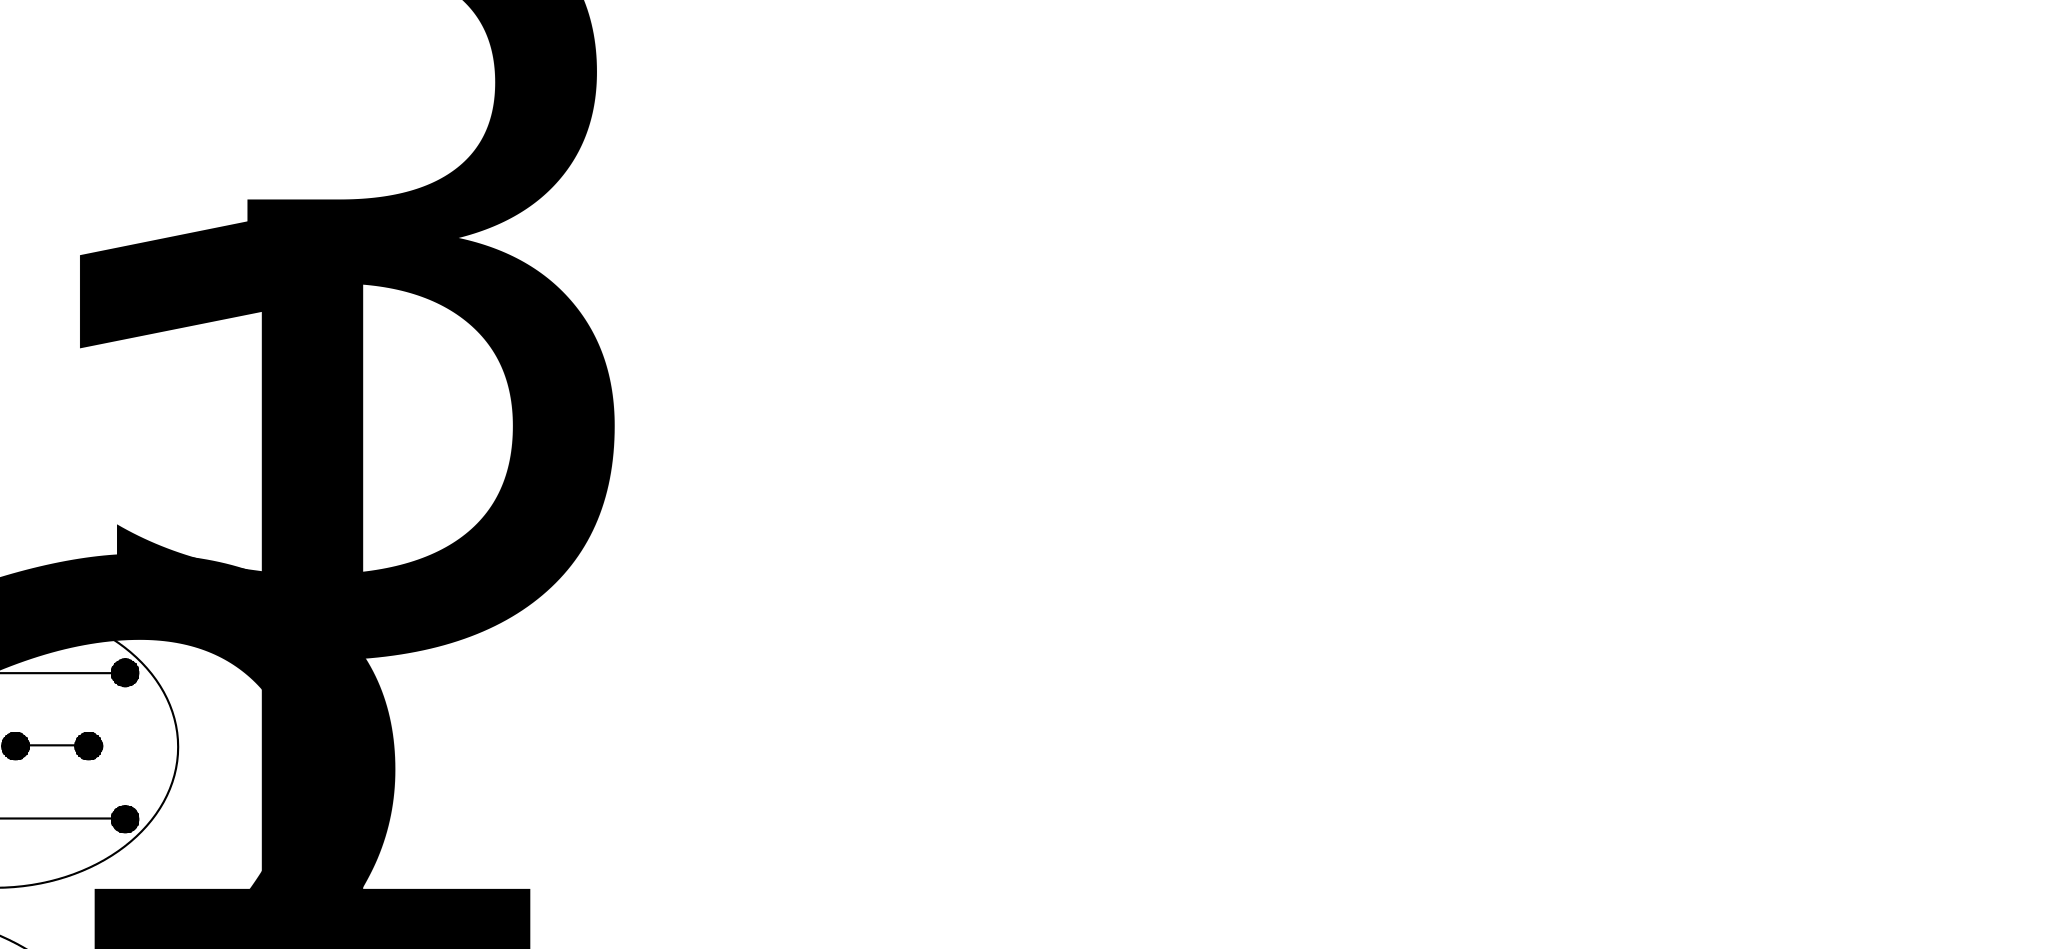
\includegraphics[height=\myMinHeight]{../../img/epsfromtikz/demo_graph}
%     \caption{}\label{fig:demo_graph:graph}
%   \end{subfigure}%
%   %
%   \hfill
%   \begin{subfigure}{0.3\linewidth}\centering
%     \includegraphics[height=\myMinHeight]{../../img/epsfromtikz/demo_graph_comdrp}
%     \caption{}\label{fig:demo_graph:comdrp}
%   \end{subfigure}%
%   %
%   \hfill
%   \begin{subfigure}{0.3\linewidth}\centering
%     \includegraphics[height=\myMinHeight]{../../img/epsfromtikz/demo_graph_candrp}
%     \caption{}\label{fig:demo_graph:candrp}
%   \end{subfigure}%
%   %
%   \caption{(\ref{fig:demo_graph:graph}) A simple graph, $G_{\Delta}$, used to illustrate concepts throughout this and the next section. (\ref{fig:demo_graph:comdrp}) The complete DR-plan of $G_{\Delta}$, i.e.\ $ComDRP(G_{\Delta})$. Dashed lines indicate that the children repeat the same pattern as the others shown on this level. The children of triangles (3 edges) are omitted. (\ref{fig:demo_graph:candrp}) The canonical DR-plan of $G_{\Delta}$, which is optimal (see Section~\ref{sec:DRP}), i.e.\ $OptDRP(G_{\Delta})$. The children of triangles or omitted.}
%   \label{fig:demo_graph}
% \end{figure*}%

% \begin{figure*}\centering%
%   %
%   \includegraphics[width=0.3\linewidth]{../../img/epsfromtikz/demo_graph_candrp_seq}
%   \caption{The sequential canonical DR-plan of $G_{\Delta}$ from Figure~\ref{fig:demo_graph:graph}, which is optimal (as explained in the proof of Theorem~\ref{theorem:algo_complexity}). The children of the triangle are omitted. Compare to to the typical canonical DR-plan shown in Figure~\ref{fig:demo_graph:candrp}. Also, note that the bottom-left node, the triangle $bce$, is the intersection of the 3 children of $G_{\Delta}$ in $ComDRP(G_{\Delta})$, shown in Figure~\ref{fig:demo_graph:comdrp}.}
%   \label{fig:demo_graph:candrpseq}
% \end{figure*}%


To find the canonical DR-plan of an isostatic graph, we first need the following subroutine.

% \begin{theorem}\label{theorem:algo_find_wcvmps_complexity}
%     There exists an $O(|V|^2)$ time complexity algorithm to find the set of isostatic vertex-maximal proper subgraphs (the \dfn{clusters}) of an isostatic input graph.
% \end{theorem}

% \begin{proof}
%     Call the input graph $G=(V,E)$.
%     % If the input is not isostatic (i.e.\ does not satisfy $|E| = 2|V|-3$), run the component pebble game algorithm
%     Take an arbitrary edge $e\in E$. Run the component pebble game algorithm \cite{Jacobs:1997:PG} on the subgraph $G\setminus e$, which takes time $O(|V|^2)$. The output of this will be all of the maximal isostatic components of $G\setminus e$, which we will call the list of candidate-clusters, or $CC$. It will contain at most $|E|-1 = O(|V|)$ elements.

%     The next step is to isolate the set of true-clusters. Begin by initializing the list true-clusters, or $TC$, as an empty list. Then, for each subgraph $C\in CC$, run the \frontier\ algorithm \cite{hoffman2001decompositionII} \cite{lomonosov2004graph} on $C+e$ to find $D$ (which is the minimal isostatic subgraph containing $C+e$.) In case 1, where $D=G$, $C$ is removed from $CC$ and added to $TC$. In case 2, where $D\subsetneq G$, for all $H\in CC$ that are subgraphs of $D$, $H$ is removed from $CC$; then $D$ is added to $TC$. If every element in $CC$ results in case 1, add $e$ to $TC$. Thus, we do $O(|V|)$ work on $O(|V|)$ subgraphs for a total time of $O(|V|^2)$.
% \end{proof}

\begin{theorem}\label{theorem:algo_find_wcvmps_complexity}
    There exists an \complexityAllClustersV\ time complexity algorithm to find the set of isostatic vertex-maximal proper subgraphs (the \dfn{clusters}) of an isostatic input graph.
\end{theorem}

\begin{proof}
    Call the input graph $G=(V,E)$. Initialize the empty list of current-clusters, or $CC$. For each edge $e\in E$, run the component pebble game algorithm \cite{Jacobs:1997:PG} on the subgraph $G\setminus e$. The output of this will be all of the maximal isostatic components of $G\setminus e$, which we will call potential-clusters, or $PC$. Remove any element from $PC$ that is a subgraph of an element in $CC$, then remove any element from $CC$ that is a subgraph of an element in $PC$. Add all remaining elements of $PC$ to $CC$. Return $CC$ after running all edges.

    The time complexity is $O(|V|^3)$. For each edge, of which there are $O(|V|)$, we run the component pebble game, which takes $O(|V|^2)$, and then check its $PC$ against the $CC$, which also takes $O(|V|^2)$. This subgraph comparison can be done by labeling each edge in $E$ with a pointer to the element that contains it in $PC$ and $CC$ while running the component pebble games. Then, traverse edge set $E$ and check if the corresponding elements of $PC$ and $CC$ are subgraphs.
\end{proof}

\begin{figure*}\centering%
  %
  \includegraphics[width=0.3\linewidth]{../../img/svg/3xc2c3_candrp_seq}
  \caption{The sequential canonical DR-plan of $G_{demo}$ from Figure~\ref{fig:demo_graph:graph}, which is optimal (as explained in the proof of Theorem~\ref{theorem:algo_complexity}). The children of the triangle are omitted. Compare to to the typical canonical DR-plan shown in Figure~\ref{fig:demo_graph:candrp}. Also, note that the bottom-left node, the triangle, is the intersection of the 3 children of $G_{demo}$ in $ComDRP(G_{demo})$, shown in Figure~\ref{fig:demo_graph:comdrp}.}
  \label{fig:demo_graph:candrpseq}
\end{figure*}%

\begin{theorem}\label{theorem:algo_complexity}
    There exists an \ComplexityCanDRPV\ algorithm to find a canonical DR-plan for an independent input graph.
\end{theorem}

\begin{proof}
    Call the input graph $G=(V,E)$. We will call the result of the algorithm $CanDRP(G)$.

    If $G$ is a single edge, return $G$.

    % Either $G$ is isostatic (i.e.\ satisfies $|E|=2|V|-3$)
    If $G$ is not isostatic (i.e.\ does not satisfy $|E|=2|V|-3$), run the component pebble game on $G$ to get the set of isostatic vertex-maximal subgraphs. Return the forest formed by recursively running $CanDRP$ on each element.

    If $G$ is isostatic, run the isostatic vertex-maximal proper subgraph detection algorithm (Theorem \ref{theorem:algo_find_wcvmps_complexity}) on $G$ to get what we call the list of clusters. This can be done in \complexityAllClustersV\ time. Choose two arbitrary clusters, called $C_1$ and $C_2$. If $C_1\cap C_2$ is trivial (a single vertex), recursively apply $CanDRP$ on all clusters and set the results as the children of $G$; return $G$. Else if $C_1\cap C_2$ is non-trivial (an isostatic subgraph), apply $CanDRP$ to $C_1$ (note that this choice is still arbitrary, any cluster will suffice) and $T$ (the underconstrained graph formed by $C\setminus C_1$ together with all incident edges and the associated vertices in $C$) and set the results as the children of $G$; return $G$.

    For the sake of increased clarity (and performance in implementation), we expand on the case of isostatic input with clusters that intersect non-trivially. Instead of immediate recursive application of $CanDRP$, we propose an equivalent method to first compute the decomposition down to $I=\bigcap_{k=1}^{N}{C_k}$. (The rationale and nomenclature is discussed in detail in the proof of Theorem \ref{theorem:main}.) Let $R_i= C\setminus C_i$; note that each $R_i$ is pairwise disjoint. Let $T_i$ be $R_i$ plus all incident edges; note that these edges are incident on vertices in $I$ and that $T_i$ is underconstrained. Let $S_i = C\setminus \bigcup_{j=1}^{i}{R_j}$. Set the children of $G$ as $S_1=C\setminus R_1=C_1$ and $CanDRP(T_1)$. Set the children of $S_1$ as $S_2=C\setminus (R_1\cup R_2)$ and $CanDRP(T_2)$. Etc. At step $N$, set the children of $S_{N-1}$ as $CanDRP(S_N)$ and $CanDRP(T_N)$. Thus we can avoid the $N$ recomputations of the isostatic components of $G$.

    We call this intermediate result of the algorithm the ``sequential'' canonical DR-plan. See Figure~\ref{fig:demo_graph:candrpseq} for an example. This plan is a tree, where each node is a distinct subgraph, each is smaller than its parent, and the leaves comprise the edge set of $G$. Therefore, the number of nodes in the tree is $O(|E|)$ which, for independent input graphs, is $O(|V|)$. The cluster finding algorithm is run on each internal node, resulting in an overall time complexity of \ComplexityCanDRPV.

    The sequential canonical DR-plan can then be used to find the canonical DR-plan in
    % sub-cubic
    sub-quartic
    time. Simply alter any subtree that is the result of non-trivial intersection in the obvious way (adding nodes for the clusters implied by the decomposition) to get the canonical DAG. Although, in practice, the sequential plan may be sufficient.
    %
    % \note In the best case, this can be $O(V^2)$ if the graph is a 2-tree
\end{proof}


% Note that in the case of each stage of decomposition resulting in trivial intersections, this algorithm can be run in time $O(|V|^3)$. We can find all clusters in time $O(|V|^2)$, because we only have to look at a constant number of edges. Take two arbitrary edges to get the two sets of potential-clusters, $PC_1$ and $PC_2$.



% \begin{proof}
%     Choose an arbitrary ordering of the edges, such that $e_i$ is the $i^\text{th}$ edge in the sequence.

%     Run component pebble game on each edge to get the map $M$ that takes an edge, $e$, and returns a set of subgraphs that are the output of the component pebble game on $G\setminus e$. On each run of the pebble game, also attach a pointer to each edge that points to the subgraph containing the edge.
%     Call this map $P$, where $P(i, j)$ (which is not defined where $i=j$) returns a pointer to the element containing $e_i$ from $M(e_j)$.
%     This is $O(|V|^3)$.

%     Dropping an edge will never result in some other edge being in some new cluster, the other edge will only ever be in a subset of its true cluster. Therefore, we can look at each edge in $E$ and find the proper maximal subgraph containing it by following all the cluster pointers and comparing the cardinality of the vertex sets, taking the largest. This can be done in $O(|V|^2)$. Save any subgraph found in this manner.
%     HAVE TO CHECK FOR DUPLICATES... CAN BE ROLLED INTO NEXT STEP, DIFFERENT BASED ON INTERSECTION TYPE. JUST DO AN EDGE FROM THE COMPLEMENT ($G\setminus C$) SECOND.

%     Now check the intersections between clusters (pick an arbitrary two).

%     In the case of trivial intersections, all of the found clusters will be edge-disjoint.
%     For each cluster $C$, take the submatrix of $P$ only on the intersections of elements in $C$. That is, if $C$ contains $i$ and $j$, keep element $P(i,j)$. Delete any element in $M$ whose pointer is lost from $P$ after this operation.
%     % For each edge $e_i$, for every edge $e_j$ not in the cluster to which $e_i$ belongs, delete $P(i, j)$ and the element it points to in $M(e_j)$ (if it isn't already deleted).
%     This can be done in $O(|V|^2)$ time.
%     The result will be a new $P$ and $M$ for each cluster, containing only the edges in the cluster. Furthermore, all clusters from this stage will be removed from $M(e_i)$ (for all $i$).
%     % Divide the edges into sets based on their containing cluster (one edge is contained in only one cluster) and repeat the previous step.
%     Recursively run the algorithm on these clusters, but we can now skip the first step, avoiding $O(|V|^3)$ work at each node... So with an initial step of $O(|V|^3)$ and then $O(|V|^2)$ work at $O(|V|)$ nodes we get an overall complexity of $O(|V|^3)$.

%     In the case of isostatic intersections, you will find 2 clusters (the one with the most vertices, $C_1$, and the largest one containing the vertex set omitted from the first, $C_2$). You will also need to be careful of different clusters with the same size (just be aware it might happen, shouldn't affect anything, we'll want them later). Go to an arbitrary edge not in $C_1$. Look at the clusters containing the edge with the largest cardinality. The largest will be $C_2$, ignore it. Keep going to the next largest, adding it to the list of found clusters if it has an isostatic intersection with the $C_1$. This will take $O(|V|^2)$. Now we have all of the isostatic vertex-maximal proper subgraphs, which we call $C_1, C_2, \ldots , C_N$. Compute the intersection of all of these, which we call the ``core'' or $I$. Let $R_i = G\setminus C_i$.

%     Choose an arbitrary edge $e\in I$. Take the set $M(e)$, remove all elements that are subgraphs of $I$. Of the remainder, the elements that are subgraphs of $R_i$ are the first level of decomposition of $R_i$ and we call this subset $T_i$. Now we are ready to build the ``sequential'' canonical DR-plan of $G$ down to node $I$.

%     Set the children of $G$ as $S_1=C\setminus R_1=C_1$ and the elements of $T_1$. Set the children of $S_1$ as $S_2=C\setminus (R_1\cup R_2)$ and the elements of $T_2$. Etc. At step $N$, set the children of $S_{N-1}$ as $S_N=I$ and the elements of $T_N$.

%     For node $I$ and each element of $T_1, T_2, \ldots , T_N$ in the DR-plan, get the submatrix of $P$ using the edges of the subgraph in the node, and update $M$ accordingly.
%     % For each edge $e_i$ in the core, for every edge $e_j$ not in the core, delete $P(e_i, j)$ and the element it points to in $M(e_j)$ (if it isn't already deleted).

%     The sequential canonical DR-plan can then be used to find the canonical DR-plan in
%     sub-cubic
%     % sub-quartic
%     time. Simply alter any subtree that is the result of non-trivial intersection in the obvious way (adding nodes for the clusters implied by the decomposition) to get the canonical DAG. Although, in practice, the sequential plan may be sufficient.
% \end{proof}

First, we remind the reader of the component pebble game~\cite{Jacobs:1997:PG}. Given an independent input graph $G$ with vertex weight 2 and edge weight 1, the output will be all of the 2D maximal isostatic subgraphs. We will denote this algorithm with $COMPONENTS(G)$. For independent input, this runs in time $O(|V|^2)$.

We also introduce the term \dfn{clusters} of graph $G$ to refer to the set of isostatic vertex-maximal proper subgraphs of $G$.

Next, we define an operation called \dfn{modularization}. The function $MZ(M, I)$ takes a square matrix $M$ and a set of indices $I$ and returns $(M', A)$. $M'$ is the square matrix formed by keeping all elements $M_{ij}$ if $i,j\in I$. $A$ is the set of elements $M_{ij}$ and $M_{ji}$ where $i\in I$ and $j\notin I$.
% This operation takes $O(|I|^2)$.

% Next, we make the observation that dropping an edge will only cause other edges in the graph to be in components (as found by pebble games) that are subgraphs of their cluster ()

% Consider dropping edge $e_i$ and looking at the effect on $e_j$. In the case that all clusters intersect trivially, no edge is in multiple clusters. Therefore, $e_i$ could come from a different cluster than $e_j$, in which case dropping $e_i$ only affects its own cluster. Or $e_i$ could come from the same cluster as $e_j$, in which case all other clusters are found as components, but additionally edge-disjoint subgraphs of this cluster will be found as components.
% In the case that clusters intersect non-trivially, edges do com from multiple clusters.

\begin{proof}
    %% INITIALIZATION
    Let the input be $G=(E,V)$. If the input is an edge, terminate. If the input is not isostatic, set the roots of the forest as $COMPONENTS(G)$ then recursively call the algorithm on each root. Otherwise, do the following.

    Choose an arbitrary ordering of the edges, such that $e_i$ is the $i^\text{th}$ edge in the sequence.
    Initialize a map $M$ and a map $P$. For each $i$, set $M(e_i)=COMPONENTS(G\setminus e_i)$ and, for all $j\neq i$, set $P(i,j)$ as a pointer to the element in $M(e_i)$ whose subgraph contains $e_j$. This initialization takes time $O(|V|^3)$.


    %% STEP 1: Find the clusters
    % Choose some $i\leq |E|$, then find the
    Now we want to find the clusters of $G$.
    For each $i$, if we have not already found a cluster containing $e_i$, then find the $j$ such that $P(j,i)$ points to the component with the largest cardinality and add it to the list of clusters. This takes time $O(|V|^2)$. In the case that the clusters intersect trivially, we will find all of the clusters. In the case that they intersect non-trivially, we will find exactly two clusters. We will return to the latter case after continuing the proof for the former.

    %% STEP 2a: Trivial intersections
    In the case of trivial intersections, all of the found clusters will be edge-disjoint. For each cluster edge set $C_i$, compute $MZ(P, C_i)=(P_i, A_i)$. For element in each $A_i$, delete the component it points to in $M$. This can be done in $O(|V|^2)$ time.
    Note that, for any $i$, $M(e_i)$ contained only subgraphs of the cluster containing $e_i$ and the other clusters. By doing the deletions, we have removed all of the clusters found in this stage. This means $M$ can now be broken into an $M_i$ for each $C_i$, where $M_i$ contains only proper subgraphs of $C_i$. Now the algorithm can be run recursively on each $C_i$, while avoiding the recomputation of $M$ and $P$ by using the $M_i$ and $P_i$ we found.

    %% STEP 2b: Non-trivial intersections
    In the case of non-trivial intersections, we have only found 2 clusters (the one with the most vertices, $C_1$, and the largest one containing the vertex set omitted from the first, $C_2$) and we need to find the remainder. Go to an arbitrary edge $e_i\notin C_1$. For all $j\neq i$, if the component pointed to by $P(j,i)$ intersects non-trivially with $C_1$ add it to the list of clusters (ignore duplicates). This will take $O(|V|^2)$. Now we have all of the isostatic vertex-maximal proper subgraphs, which we call $C_1, C_2, \ldots , C_N$. Let $I=\bigcap_{k=1}^{N}{C_k}$. Let $R_i = G\setminus C_i$.
    Let $T_i = COMPONENTS(R_i)$. All of these can be computed in $O(|V|^2)$.

    % Choose an arbitrary edge $e\in I$. Take the set $A=M(e)$, remove all elements from $A$ that are subgraphs of $I$. For each $R_i$, find the set $T_i$ which contains the elements of $A$ that are subgraphs of $R_i$. Note that $T_i=COMPONENTS(R_i)$, and will be the first level of decomposition of $R_i$ since it is underconstrained.
    % COULD WE JUST RUN $COMPONENTS$???

    Now we build the ``sequential'' canonical DR-plan of $G$ down to node $I$.
    Set the children of $G$ as $S_1=C\setminus R_1=C_1$ and the elements of $T_1$. Set the children of $S_1$ as $S_2=C\setminus (R_1\cup R_2)$ and the elements of $T_2$. Etc. At step $N$, set the children of $S_{N-1}$ as $S_N=I$ and the elements of $T_N$.
    For each node $N$ of the DR-plan in the set $\{I\}\cup T_1\cup T_2\cup \cdots\cup T_N$, compute $MZ(P, N)=(P', A')$ and update $M$ by deleting all elements pointed to by $A'$. Then, for each $N$, run the algorithm recursively on (avoiding recomputation of $M$ and $P$).
    % For node $I$ and each element of $T_1, T_2, \ldots , T_N$ in the DR-plan, compute $MZ(P, \cdot)$, update $M$ in the same fashion as above, and run the algorithm recursively on $(\cdot)$ (avoiding recomputation of $M$ and $P$).

    %% Proof of complexity
    The decomposition will ultimately terminate as a tree with $|E|$ leaves, each containing a unique edge. With an initial step of $O(|V|^3)$ and then $O(|V|^2)$ work at $O(|V|)$ nodes we get an overall complexity of $O(|V|^3)$.

    The sequential canonical DR-plan can then be used to find the canonical DR-plan in
    sub-cubic
    % sub-quartic
    time. Simply alter any subtree that is the result of non-trivial intersection in the obvious way (adding nodes for the clusters implied by the decomposition) to get the canonical DAG. Although, in practice, the sequential plan may be sufficient.
\end{proof}




% In the case of trivial intersections, all of the found clusters will be unique. If the cardinality is greater than 2, we can save computation by not checking the other edges in the found cluster. But we can only know that they are trivial intersections after finding 2 different clusters. So do that first...

% In the case of isostatic intersections, if we begin with an edge in the core, there are several clusters containing this edge (and the algo will pick the largest among them). We could only safely skip the other edges in the core, but we don't know what it is yet. So after finding the first cluster, go to an edge not in it and find the next cluster. Check the intersection. Now we can skip the others in the core. WAIT.... THIS WILL ONLY PICK THE LARGEST, AND ITS ``COMPLEMENT'', SO TO SPEAK. WHICH TECHNICALLY WORKS....

% For each found cluster $c$, for each edge $e$ \emph{not in} $c$, delete $c$ from $M(e)$ and delete the pointer to $M(e)$ from the pointer list of $e$.






% \begin{proof}
% The first step of the algorithm is finding the isostatic vertex-maximal proper subgraphs of the input isostatic graph $G$. Do this by first dropping arbitrary edge $e$ from the edge set and running the pebble game algorithm \cite{Jacobs:1997:PG} on this subgraph, which is $O(|V|^2)$. The output of this will be a list of component-candidates. Then run the \frontier\ algorithm \cite{hoffman2001decompositionII} \cite{lomonosov2004graph} ($O(|V|)$) on each candidate along with edge $e$, which will find the minimal subgraph $D$ that contains the candidate and $e$. If $D=G$, move $D$ to the true-cluster list and remove the candidate from the candidate-component list. If $D\subsetneq G$, check the union of $D$ with the all items in the true-cluster list; if the union is isostatic, halt and output just these two components as children. Otherwise, remove all candidates that are subgraphs of $D$ from the candidate-component list and add $D$. Continue with the next candidate. If you exhaust the candidates, output the entire true-cluster list.

% %on the children
% This is run recursively on each node. If you use dynamic programming to store the decompositions of each component, it prevents repetition of work (done by using the DAG representation of the DR-plan). In this case you will have to do work on no more than $O(|V|)$ nodes that get smaller at each level.

% Thus, the running time is at most $O(|V|^3)$. \todo{does this amortize correctly?}

% It's a tree in only trivial case -> O(V), always order of leaves
% If its isostatic intersection, we do the sequential extension,intersections only done once.

% inductively. The number of nodes at this level will e more than the total. Number of leaves (terminals for dag) is at most the number of edges

% \end{proof}

% \begin{proof}
% The first step of the algorithm to find an optimal DR-plan is the most difficult --- to find the wellconstrained vertex-maximal proper subgraphs of the input wellconstrained graph. There are two approaches: (1) the bottom-up approach, using the \frontier\ algorithm \cite{Oung:2001:FFE:376957.376995} to grow these components from single vertices; and (2) the top-down approach, using the pebble game algorithm \cite{Jacobs:1997:PG} on each node and taking the largest components that are not subgraphs of any larger ones. After the subgraphs have been found, it is a straightforward application of the theory. If the intersection of any two of the subgraphs is wellconstrained, then take those two to be children of the graph. Otherwise, all the subgraphs are the children. Apply recursively to the children. This naturally terminates when you reach trivial subgraphs. The complexity of this depends on the algorithm for finding children (both are polynomial) and the depth of the plan (the deeper the plan, i.e.\ the smaller the max fan-in, the longer the running time). \todo{Think more about complexity.}
% \end{proof}


% \begin{figure*}\centering%
%   \includegraphics[width=\linewidth]{../../img/svg/overconstrained_choices}
%   \caption{The first graph is over constrained by one edge (a $K_{3,3}$ with an extra vertex attached by 3 edges). The second graph is a minimally rigid subgraph of the first. Any DR-plan of this graph will have fan-in of at least 9, occurring at the node that decomposes the $K_{3,3}$. The third graph is a different subgraph of the first. A canonical and cluster minimal DR-plan of size 2 can be made for this graph (it is a Henneberg-I construction). Thus, we can see the first graph has both non-optimal (second graph) and optimal (third graph) canonical, cluster minimal DR-plans.}
%   \label{fig:overconstrained_choices}
% \end{figure*}%




\ClearMyMinHeight
\SetMyMinHeight{.6}{../../img/svg/new_overconstrained_not_optimal}
\SetMyMinHeight{.4}{../../img/svg/new_overconstrained_optimal}

\begin{figure*}\centering%
    %
    \begin{subfigure}{0.5\linewidth}\centering
        \scalebox{1}[.9]{
        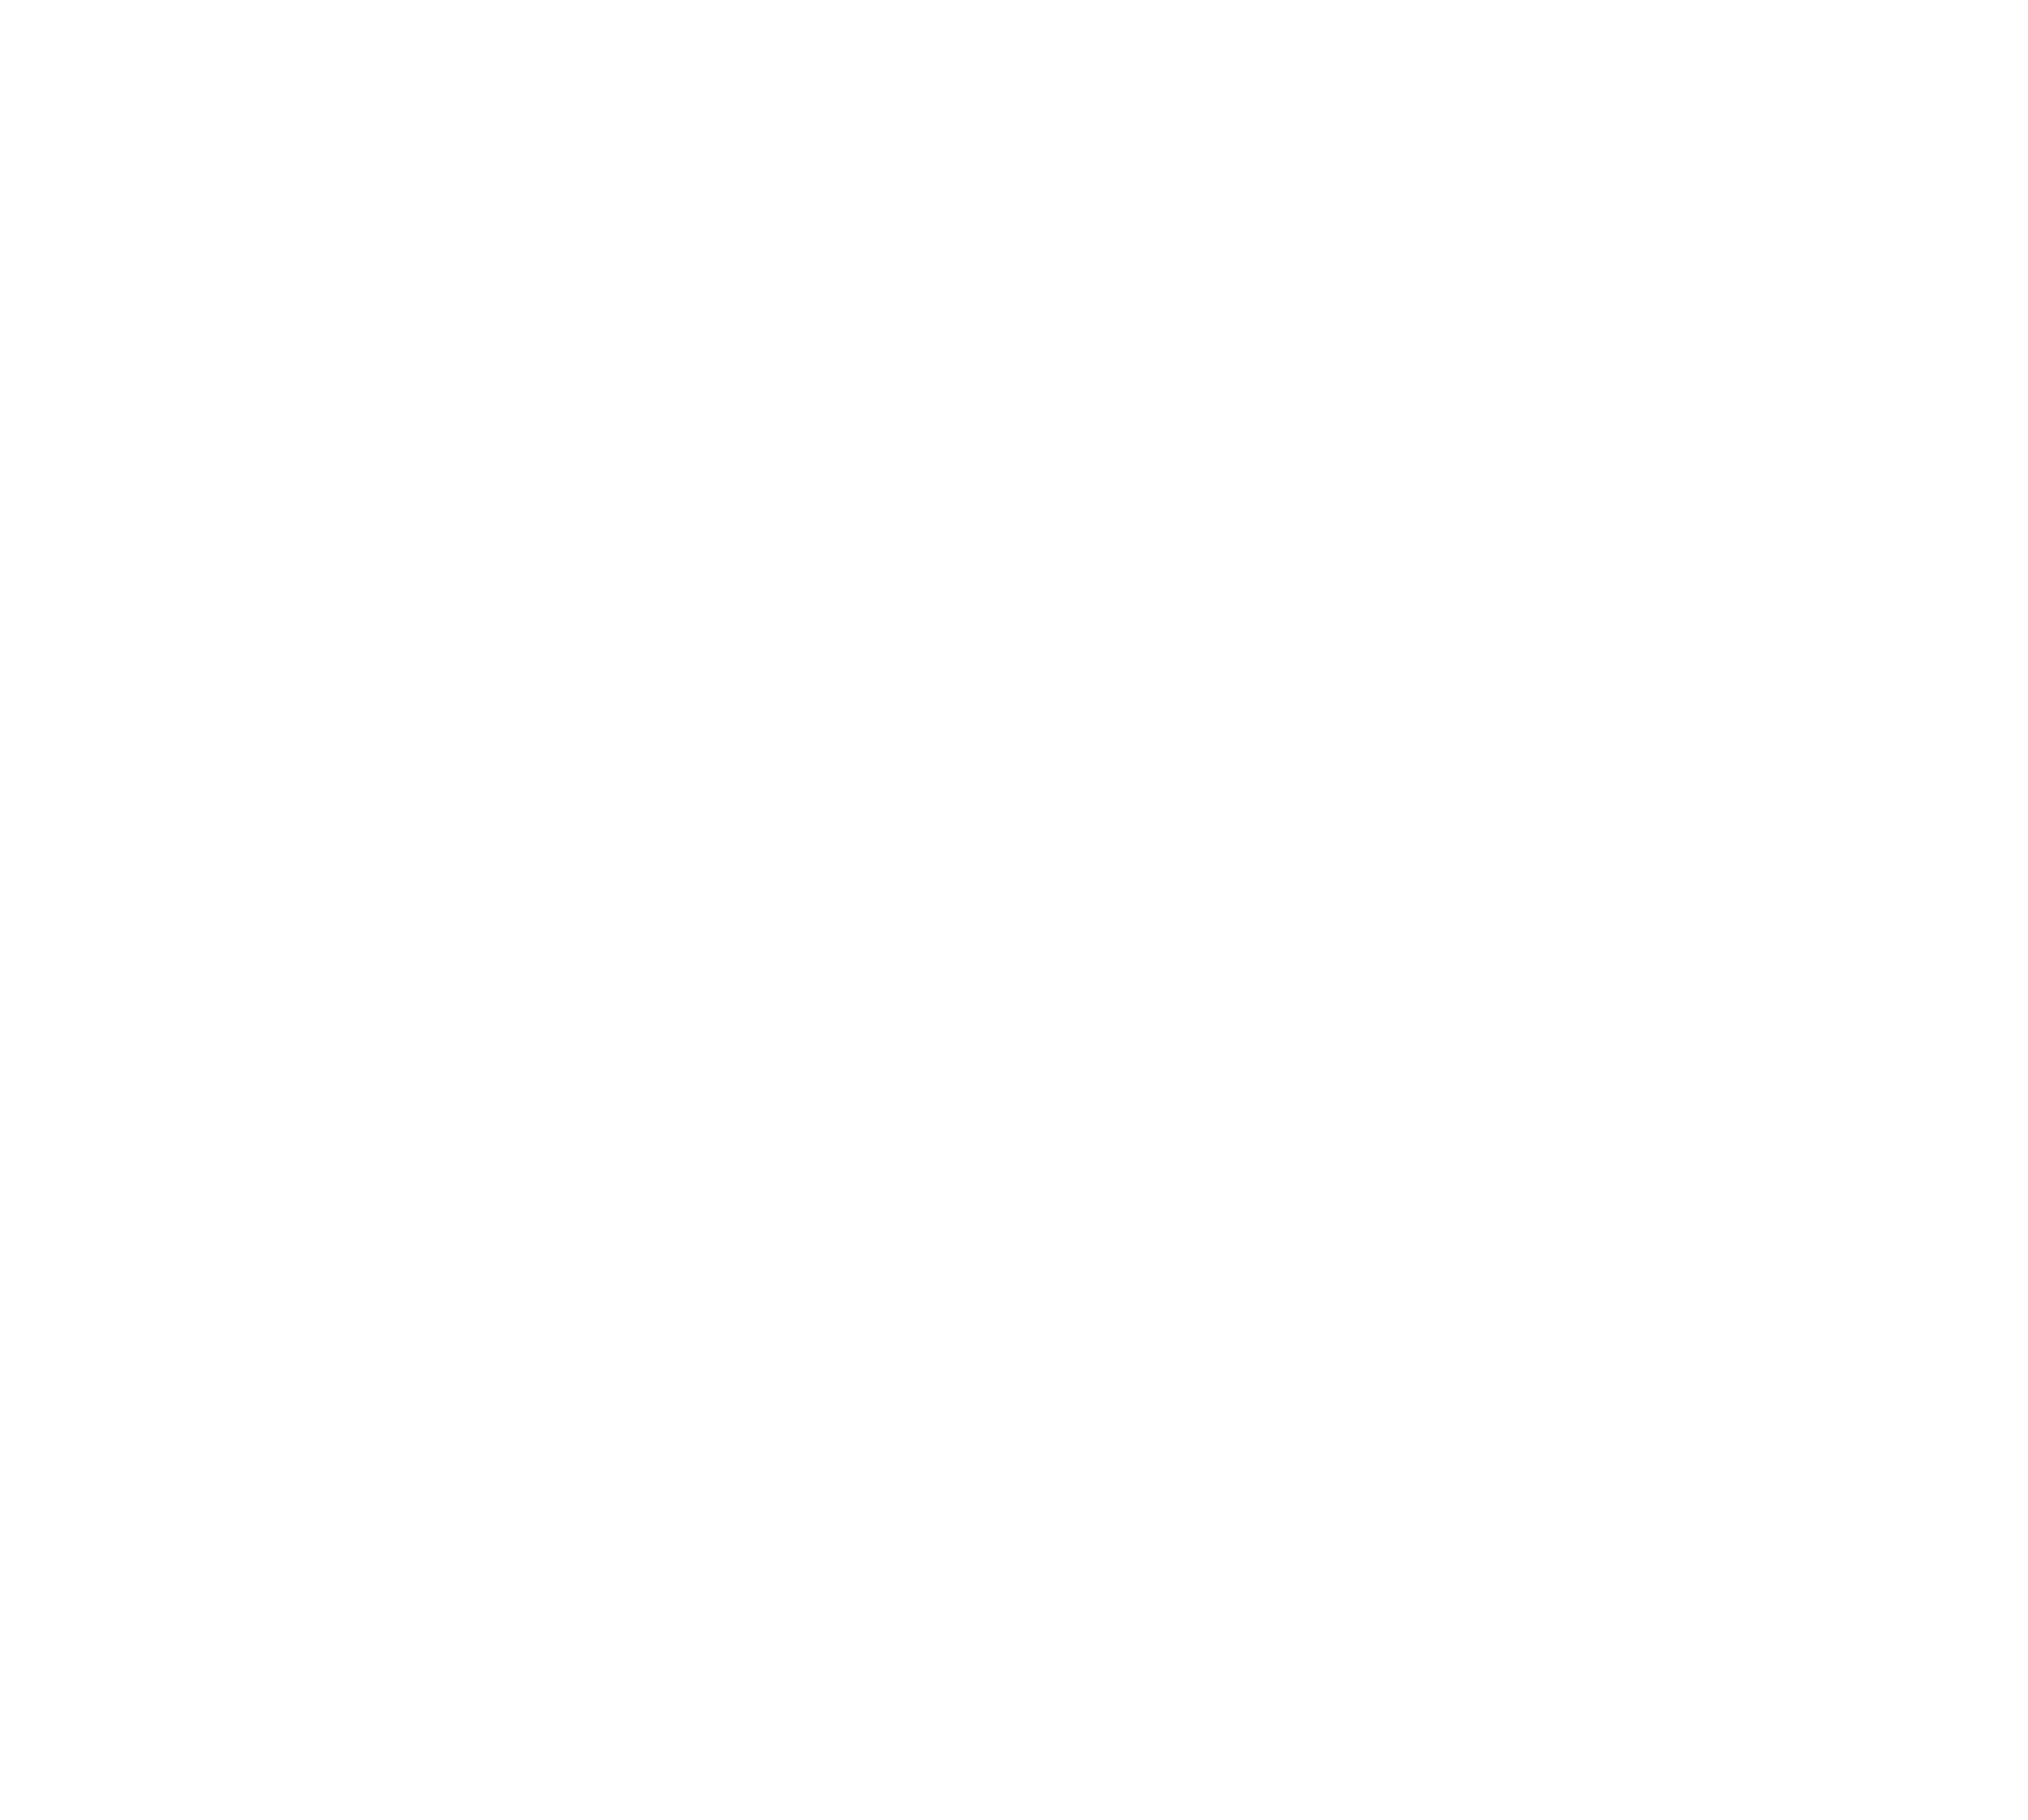
\includegraphics[height=\myMinHeight]{../../img/svg/new_overconstrained_optimal}
        }
        \caption{}\label{fig:overconstrained:optimal}
    \end{subfigure}%
    %
    \hfill
    \begin{subfigure}{0.5\linewidth}\centering
        \scalebox{1}[.9]{
        \includegraphics[height=\myMinHeight]{../../img/svg/new_overconstrained_not_optimal}
        }
        \caption{}\label{fig:overconstrained:not_optimal}
    \end{subfigure}%
    %
    \caption{
    % (\ref{fig:overconstrained:optimal}) An optimal DR-plan of a singly overconstrained rigid graph with a fan-in of 5. Decomposition of triangles is omitted. (\ref{fig:overconstrained:not_optimal}) A canonical and cluster-minimal DR-plan of the same graph. The DR-plan has a fan-in of 9 and is non-optimal, shown by the preceding counter-example. Since the nontrivial intersection of the two children of the root is underconstrained, their decompositions are separate, causing the large fan-in.
    Both figures are canonical and cluster-minimal DR-plans of the same singly overconstrained rigid graph. Decomposition of triangles are omitted and dashed lines indicate a decomposition similar to the other nodes on the same level. (\ref{fig:overconstrained:optimal}) is an optimal DR-plan, with a fan-in of 5. (\ref{fig:overconstrained:not_optimal}) has a fan-in of 9 and is non-optimal, shown by the preceding counter-example.
    }
    \label{fig:overconstrained}
\end{figure*}%

\subsection{Overconstrained Graphs and NP-Hardness of Optimal DR-Planning}
\label{sec:drp:overconstrained}

For overconstrained (not independent) graphs, a canonical DR-plan is still well-defined.
However, it may be far from optimal. The proofs of Theorem \ref{theorem:main}, Observation \ref{lemma:union_intersection}, and Lemma \ref{lemma:combined_lemma} all fail for overconstrained graphs.
It is important to note that, regardless whether the graph is overconstrained, if every node in a canonical DR-plan $R$ has clusters whose pairwise intersection is trivial, then the DR-plan is the unique one satisfying Property (2), and since we know that there is an optimal DR-plan that satisfies Property (2), $R$ is in fact optimal. The problem arises when some node in a DR-plan has clusters whose pairwise intersection is non-trivial.
In this case, an arbitrary choice of a pair of clusters as children of an overconstrained node in a canonical DR-plan may not result in an optimal DR-plan. This is in contrast to independent graphs, which, as shown in Theorem~\ref{theorem:main}, exhibit the strong Church-Rosser property that any choice yields an optimal DR-plan.
% \todo{rephrase? Theorem 4 shows this. If it's independent it \vemph{will} be optimal (the church rosser property), no longer holds if it's overconstrained.}
A good source of examples of overconstrained graphs with canonical DR-plans that are not optimal are graphs whose cluster-minimal DR-plans that are not optimal. The example shown in Figure \ref{fig:overconstrained} is a canonical, cluster-minimal DR-plan that is not optimal; an optimal DR-plan is also shown in the figure.
The root cause of the NP-hardness is encapsulated in this figure: because the different choices of vertex-maximal subgraphs for overconstrained input do not incur the same fan-in, finding the optimal DR-plan becomes a search problem with a combinatorial explosion of options.


As mentioned earlier, the Modified \frontier\ algorithm
version given in \cite{lomonosov2004graph} runs in polynomial time and finds a cluster-minimal DR-plan for any graph.
Similarly, the algorithm given above finds a canonical DR-plan also for any input graph.  However neither of these DR-plans may be optimal for overconstrained graphs as shown in Figure \ref{fig:overconstrained}.

While the canonical DR-plan is optimal only if the input graph is independent, when there are only $k$ overconstraints for some fixed $k$, we can still find the optimal DR-plan using a straightforward modification of the above algorithm. However, the time complexity is exponential in $k$.

This exponential growth of time complexity for overconstrained graphs is in fact captured in the proof of NP-hardness of optimal DR-planning in \cite{sitharam2005combinatorial, lomonosov2004graph}.
